% Illustrative accepted task: T_i=3 days, tau=14 days, Delta=14 days.
% Hence requirement assessment is at day 17, and the labour total includes work through day 28.
% Text alternative: acceptance by day fourteen qualifies its weighted score for inclusion;
% its day-three acceptance starts fourteen-day follow-up. Labour is counted
% from day zero through day twenty-eight, including work after the requirement assessment.
\begin{figure}[htp]
\centering
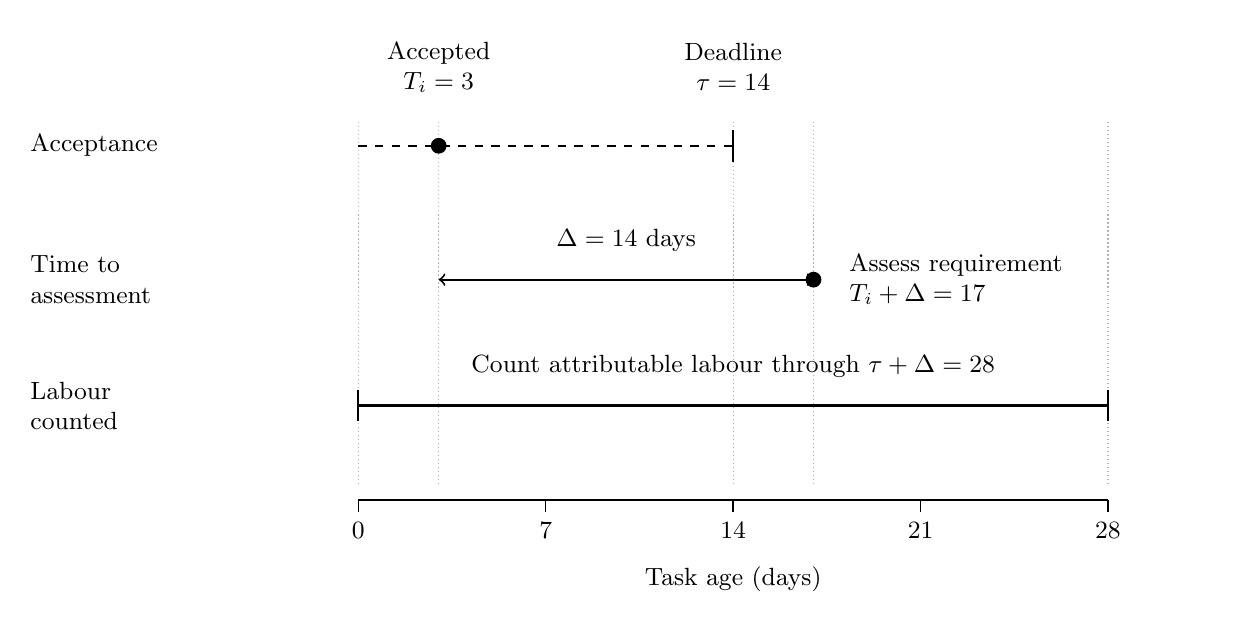
\begin{tikzpicture}[x=1mm,y=1mm,font=\fontsize{9}{11}\selectfont,
  every node/.style={inner sep=1pt,outer sep=0pt}]
  \path[use as bounding box] (0,-8) rectangle (152.4,65);
  \node[anchor=west] at (0,50) {Acceptance};
  \node[anchor=west,align=left] at (0,33) {Time to\\assessment};
  \node[anchor=west,align=left] at (0,17) {Labour\\counted};
  \foreach \day in {0,3,14,17,28} {
    \draw[black!30,densely dotted,line width=0.45pt]
      ({42+3.4*\day},7) -- ({42+3.4*\day},53);
  }
  \draw[dashed,line width=0.7pt] (42,50) -- (89.6,50);
  \fill (52.2,50) circle (1mm);
  \draw[line width=0.7pt] (89.6,48) -- (89.6,52);
  \node[align=center] at (52.2,60) {Accepted\\$T_i=3$};
  \node[align=center] at (89.6,60) {Deadline\\$\tau=14$};
  \draw[<->,line width=0.7pt] (52.2,33) -- (99.8,33);
  \node at (76,38) {$\Delta=14$ days};
  \fill (99.8,33) circle (1mm);
  \node[anchor=west,align=left] at (104,33) {Assess requirement\\$T_i+\Delta=17$};
  \draw[line width=1pt] (42,17) -- (137.2,17);
  \foreach \xx in {42,137.2} {
    \draw[line width=0.7pt] (\xx,15) -- (\xx,19);
  }
  \node at (89.6,22) {Count attributable labour through $\tau+\Delta=28$};
  \draw[line width=0.5pt] (42,5) -- (137.2,5);
  \foreach \day in {0,7,14,21,28} {
    \draw[line width=0.5pt] ({42+3.4*\day},5) -- ({42+3.4*\day},3.5);
    \node[anchor=north] at ({42+3.4*\day},2.5) {\day};
  }
  \node at (89.6,-5) {Task age (days)};
\end{tikzpicture}
\caption{\textbf{Requirement fulfilment is assessed after acceptance, while labour is counted to a common task age.}
In this example, the task is accepted on day three and both $\tau$ and $\Delta$ are fourteen days. The fraction of its accepted requirement still satisfied is assessed on day seventeen, fourteen days after acceptance. Its labour total includes work through day twenty-eight, the common task age $\tau+\Delta$, including labour attributable to the task after its requirement assessment. The solid line marks the period over which labour is summed. Human work may occupy only part of that period. Adding $s_i$ converts task age to calendar time.}
\label{fig:task-clocks}
\end{figure}
